\chapter{Visão Geral da Arquitetura e Componentes}


\section{Fase 01}

\begin{figure}[hb]
    \begin{center}
        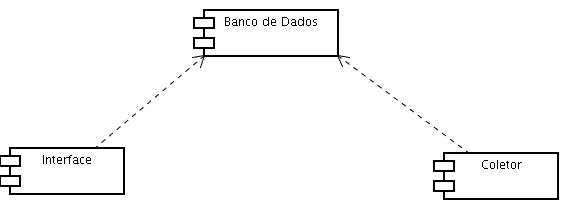
\includegraphics[scale=0.5]{img/conceitual}
        \caption{Arquitetura conceitual geral do sistema}
        \label{fig:arquitetura-conceitual}
    \end{center}
\end{figure}

\section{Fase 02}

\begin{figure}[hb]
    \begin{center}
        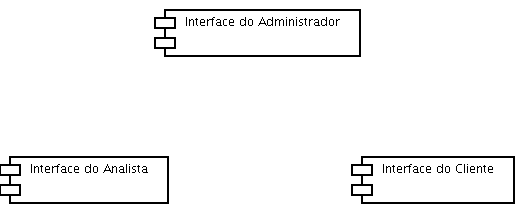
\includegraphics[scale=0.5]{img/interface}
        \caption{Arquitetura dos subsistemas da interface}
        \label{fig:arquitetura-interface}
    \end{center}
\end{figure}

\begin{figure}[hb]
    \begin{center}
        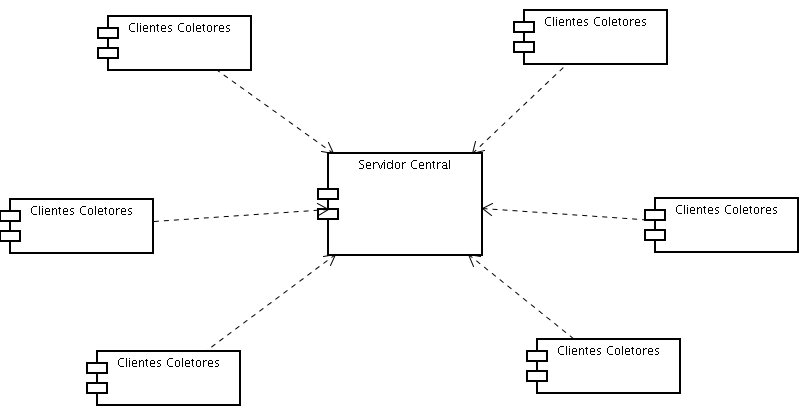
\includegraphics[scale=0.5]{img/coletor}
        \caption{Arquitetura dos subsistemas do coletor}
        \label{fig:arquitetura-coletor}
    \end{center}
\end{figure}

\section{Fase 03}

\begin{figure}[hb]
    \begin{center}
        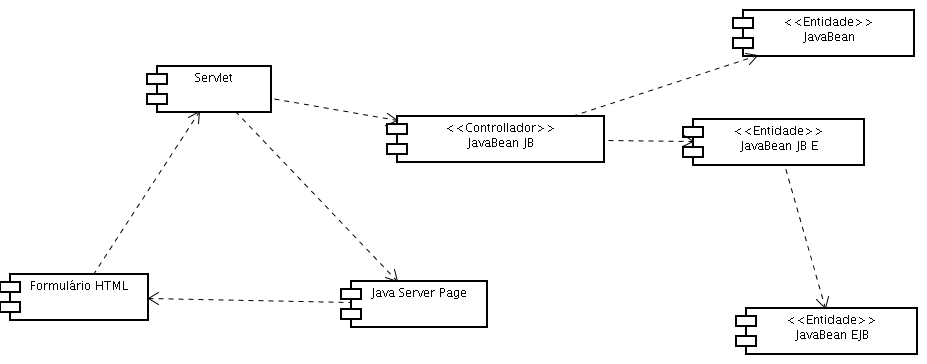
\includegraphics[scale=0.5]{img/jsp}
        \caption{Visão de camadas da implantação JSP}
        \label{fig:}
    \end{center}
\end{figure}

